\documentclass[11pt]{article}

\usepackage[margin=1in]{geometry}
\usepackage{amsmath,amsthm,amssymb}
\usepackage{booktabs}
\usepackage{longtable}
\usepackage[colorlinks=true,linkcolor=blue,citecolor=blue,urlcolor=blue]{hyperref}
\usepackage{cleveref}

% Let TeX stretch slightly to resolve minor overfull lines (long \texttt names,
% dense math) rather than clipping into the right margin. Content-neutral.
\setlength{\emergencystretch}{3em}

\newtheorem{theorem}{Theorem}
\newtheorem{proposition}{Proposition}
\newtheorem{definition}{Definition}

\title{Toward Dyson's Quasicrystal:\\ Kernel-Verified Diffraction,\\ Finite-Height Localization, and an\\ Effective Zero-Free Region for the\\ Riemann Zeta Zeros\\[0.6em] \large with the Telperion certificate engine}
\author{Peter W. Murphy, MD}
\date{\today}

\begin{document}
\maketitle

\begin{abstract}
Dyson proposed that the nontrivial zeros of the Riemann zeta function should be
understood---\emph{if the Riemann Hypothesis holds}---as a one-dimensional
quasicrystal: a point set whose diffraction spectrum is pure point, supported on
the logarithms of prime powers. The
mathematical substance of that reading is the Guinand--Weil explicit formula---the
identity under which the zeros diffract off the primes. We report a body of
kernel-verified mathematics, in Lean~4 against Mathlib, that carries the finite
part of that program: a machine-checked \emph{finite-height explicit formula}
(weighted sums over zeta's actual divisor equal von Mangoldt prime-power sums plus
three explicit boundary integrals, with the prime-side edge derived, not
certified); a complete finite Turing verification that \emph{all 3474 nontrivial
zeros up to height 4000 lie on the critical line}, band-tiled with a uniform,
documented numeric trust boundary; the \emph{Riemann--von Mangoldt counting
formula} $N(T) = \theta(T)/\pi + 1 + S(T)$, exact at finite height, with
$S$ and $\theta$ defined branch-free in the kernel; and a self-contained, \emph{effective} de la
Vallée-Poussin zero-free region ($\zeta(s) \ne 0$ on $\operatorname{Re} s > 1 -
c/\log|\operatorname{Im} s|$ with an explicit constant). \emph{We do not claim the
Riemann Hypothesis}: every statement is finite or a region, every numeric input is
an explicit hypothesis, and \texttt{conjecture1\_proved = False} is a tested
invariant of the repository. The instrument is \emph{Telperion}, a certificate
compiler built on the principle \emph{check the witness, don't trust the author}:
an untrusted generator certifies each claim in exact arithmetic and emits Lean
that Mathlib's kernel re-proves from scratch, with a self-verification layer
(sensitivity declarations, forge-the-witness negative controls, an independent
second checker) against true-but-vacuous theorems. The same engine has been
applied to open problems in extremal combinatorics and proof complexity,
reported separately.
\end{abstract}

\section{Introduction}
\label{sec:intro}

In his 2009 essay \emph{Birds and Frogs}, Freeman Dyson proposed a way of
looking at the Riemann Hypothesis that is geometric rather than analytic
\cite{dyson2009}. If RH is true, the nontrivial zeros of the zeta function form
a \emph{one-dimensional quasicrystal}: a point set that is not periodic, yet
whose diffraction spectrum is pure point---discrete spectral lines, like a
crystal's---supported on the logarithms of the prime powers. Classify the
one-dimensional quasicrystals, Dyson suggested, and one might find the zeros on
the list. The mathematical substance beneath the metaphor is not conjectural at
all: it is the Guinand--Weil explicit formula \cite{guinand1948,weil1952}, the
identity under which weighted sums over the zeros equal weighted sums over the
primes---the zeros \emph{diffracting} off the primes. Everything in the
quasicrystal picture descends from that identity, which in turn descends from
Riemann's 1859 memoir.

This paper reports a body of machine-checked mathematics---formalized in
Lean~4 and re-proved from scratch by Mathlib's kernel---that carries the
\emph{finite} part of that program, and is scrupulous about the boundary
between what is proved and what is not. Three results form the spine
(\cref{sec:rh}):
\begin{itemize}
  \item \textbf{A finite-height explicit formula, in the kernel.} For any box
    with right edge in $\operatorname{Re} s > 1$ and any holomorphic test
    weight, weighted sums over zeta's \emph{actual} meromorphic divisor equal
    von Mangoldt prime-power sums plus three explicit boundary integrals---a
    rectangular Guinand--Weil identity, the diffraction identity at finite
    height. The prime-side edge needs no numeric certificate at all: its
    non-vanishing is a theorem.
  \item \textbf{All zeros to height 4000, on the line.} A complete finite
    Turing verification: the $3474$ nontrivial zeros with
    $0 < \operatorname{Im}\rho \le 4000$ lie exactly on
    $\operatorname{Re} s = \tfrac12$, assembled from eighty-nine band
    certificates composed through an unbounded-depth height chain, their
    winding counts derived from boundary contours, with
    a uniform, documented numeric trust boundary and no bare classical
    hypothesis.
  \item \textbf{An effective de la Vallée-Poussin region.} A self-contained,
    machine-checked $\zeta(s) \ne 0$ on
    $\operatorname{Re} s > 1 - c/\log|\operatorname{Im} s|$, with $c$ an
    explicit closed-form constant---a refinement over the classically
    non-effective statement---together with elementary Hadamard-free regions
    that appear to be the first of their kind verified in Lean.
\end{itemize}
Around that spine the same section reports, at the same standard of honesty,
finite kernel-checked prefixes of two classical RH criteria (Jensen--P\'olya
hyperbolicity and Li positivity) and---asserted by Riemann in 1859, proved by
von Mangoldt, and now a theorem of the kernel---the Riemann--von Mangoldt
counting formula itself, $N(T) = \theta(T)/\pi + 1 + S(T)$, exact at finite
height.
Let us say immediately what none of this is: \emph{we do not claim the Riemann
Hypothesis}. The explicit formula is an instrument for studying RH, not a
conclusion about it; the Turing verification is finite; the zero-free region is
a region. Every numeric input enters as an explicit, documented hypothesis, and
\texttt{conjecture1\_proved = False} is a real, tested invariant of the
repository, not a slogan.

\paragraph{The instrument.} Results at this scale---hundreds of kernel-checked
theorems, many of them generated rather than hand-written---raise a trust
question. Search procedures, heuristics, and increasingly large language models
are very good at producing arguments that \emph{look} right, and the more
fluent the generator, the more convincing its mistakes. Our answer is old and
clean: \emph{check the witness, don't trust the author}. The instrument behind
every result above is \emph{Telperion}, a certificate compiler for Lean~4: you
describe a family of concrete claims, Telperion certifies each instance in
exact rational arithmetic and emits Lean, and Mathlib's kernel re-proves every
line from scratch (\cref{sec:system}). The generator is untrusted by design---a
wrong certificate is a compile error, never a false theorem. Because the kernel
cannot catch a theorem that is true but \emph{vacuous}, Telperion adds a
self-verification layer---per-emitter sensitivity declarations,
forge-the-witness negative controls, and an independent second checker---and is
honest about the one thing no machinery can settle: whether a formal statement
means the informal claim a human intended (\cref{sec:vacuity}).

\paragraph{The instrument elsewhere.} The same discipline carries to problems
far from the zeta function, and we include two of them as evidence that the
method, not the subject, is what generalizes: a machine-checked analytic core
for the (still open) Brualdi--Goldwasser tree-maximizer conjecture, where we
say exactly which bridge is missing (\cref{sec:bg}); and a kernel-checked,
symbolic-in-$n$ sum-of-squares lower bound for the Grigoriev knapsack system in
proof complexity, where the mathematics is due to others and our contribution
is the certified pipeline (\cref{sec:pc}).

\paragraph{A note on posture.} A reader will notice that we spend as much care
on what is \emph{not} proved as on what is. That is deliberate. The honesty
flags in this project are load-bearing, and a certificate engine whose whole
value is that you need not trust it would be a strange place to start
overclaiming. \Cref{sec:evaluation} takes up the limitations directly, and the
reproducibility appendix gives a reviewer the commands to re-check any claim in
this paper themselves.

\section{Main results: the zeta program}
\label{sec:rh}

This section is the paper's spine, and it comes with a warning label we want to
put first, in bold, so there is no chance of misreading: \textbf{we do not claim
the Riemann Hypothesis.} What we have is a connected body of genuine,
machine-checked results \emph{about} the zeta function---built in the order a
reader should understand them: first where the zeros \emph{cannot} be (zero-free
regions, culminating in an effective de la Vallée-Poussin region), then where
they \emph{are} (a complete finite Turing verification to height $4000$), and
finally what they \emph{mean} (the finite-height explicit formula---the
diffraction identity of Dyson's quasicrystal picture \cite{dyson2009})---with,
along the way, finite prefixes of two classical RH criteria and the
Riemann--von Mangoldt counting formula, proved in the kernel.
Each
result is stated with an honest account of how it sits relative to the classical
literature, and in every case it falls well short of the Riemann Hypothesis.

\subsection{Four verified results}

Each of the following is proved in Lean~4 against pinned Mathlib, is
\emph{unconditional}, and is guarded in continuous integration by an axiom check
(\texttt{\#print axioms} must report no \texttt{sorryAx}), so ``verified'' here is
enforced, not asserted:

\begin{enumerate}
  \item a fractional-part \emph{strip representation} of $\zeta$ on
    $\{\operatorname{Re} s > 0\} \setminus \{1\}$ (\texttt{zeta\_fract\_repr});
  \item the sharp bound $\lVert \zeta(\sigma+it) \rVert \le 6\,(1 + \log|t|)$ on
    $1 \le \sigma \le 2,\ |t| \ge 2$, with an explicit constant
    (\texttt{zeta\_log\_bound});
  \item an elementary, Hadamard-free zero-free region
    $\operatorname{Re} s > 1 - c/|t|^5$ (\texttt{riemannZeta\_zero\_free\_poly});
  \item a sharper region $\operatorname{Re} s > 1 - c/\!\left(|t|^4 (1 + \log 2|t|)\right)$
    (\texttt{riemannZeta\_zero\_free\_polylog}).
\end{enumerate}

To our knowledge, the last two are the first unconditional, Hadamard-free
zero-free regions to be machine-checked in Lean.

\subsection{The honest comparison---and a second route to the full rate}

Now the part that keeps this truthful, and it has two registers. Taken by
themselves, the four regions above are \textbf{strictly weaker than de la
Vallée-Poussin}: the classical region is $\operatorname{Re} s > 1 - c/\log|t|$
\cite{dlvp1896}, and $1/\log|t|$ beats a polynomial or polylog decay in $|t|$
handily. What is new about \emph{them} is only the \emph{formal derivation}---an
elementary, Hadamard-free route to an unconditional region in a proof assistant,
with a handful of reusable gap-fillers (the strip representation and the explicit
$\log$-bound among them).

A second, non-elementary route has since reached the full de la Vallée-Poussin
region itself---as a self-contained $\zeta(s) \ne 0$ statement, with an
\emph{effective} constant. Through a Blaschke / canonical-factor decomposition of
$\zeta$ and a box argument principle, the theorem
\texttt{riemannZeta\_ne\_zero\_region} states
\[
  |\operatorname{Im} s| \ge \tfrac{55}{16}, \quad
  \operatorname{Re} s > 1 - \frac{\mathtt{dlvpRateC}}{\log|\operatorname{Im} s|}
  \qquad\Longrightarrow\qquad \zeta(s) \ne 0,
\]
where \texttt{dlvpRateC} is not an existential but a \emph{concrete closed-form
real}---built from $\pi$ and two logarithms---made possible by an explicit pole
bound $\operatorname{Re}\!\big({-}\zeta'/\zeta(\sigma)\big) \le
\operatorname{Re}\!\big(1/(\sigma-1)\big) + 16$ that replaces Mathlib's
bare-existential pole constant. It is sorry-free (axioms $\{$\texttt{propext},
\texttt{Classical.choice}, \texttt{Quot.sound}$\}$), CI-axiom-guarded in
\texttt{AxiomGuardDlvp}, and carries no numeric or Arb hypotheses. It is the clean
top of a short ladder that is guarded in full: the zero-location bound
\texttt{dlvp\_zeta\_region\_rate\_effective}
($\beta \le 1 - \mathtt{dlvpRateC}/\log|\gamma|$ for a zero $\beta + i\gamma$), its
$\exists\,c$ predecessor \texttt{dlvp\_zeta\_region\_rate}, and the pre-rate
existential \texttt{dlvp\_zeta\_region\_concrete} whose constant hid inside an
$\exists\,A\,L$.

One honest qualification holds it to its true strength, and it is not
``conditional'': the region is stated for $|\operatorname{Im} s| \ge \tfrac{55}{16}$,
the standard large-height form. The two softnesses that appeared in intermediate
lemmas---a zero's multiplicity as an input, and a $\beta \ge \tfrac34$ window---are
now discharged \emph{internally} (the multiplicity is derived from $\zeta(\rho_0) =
0$; the window follows from $\mathtt{dlvpRateC} \le 1/1792$ and $\zeta$ having no
zeros with $\operatorname{Re} \ge 1$), so the statement itself is a clean
$\zeta \ne 0$. What it is \emph{not} is a proof of RH: we have matched the classical
dVP zero-free region---now self-contained, with an explicit, effective constant, a
refinement over the classically non-effective statement---inside a proof assistant,
but we have not improved the rate (Vinogradov--Korobov is stronger still), and a
zero-free region is not RH. The contribution, here as throughout, is the
machine-checked path---dVP is a theorem of 1896---stated at exactly its strength.

\subsection{Criterion prefixes: Jensen--P\'olya hyperbolicity and Li positivity}

The zero-free regions are not the only honestly-scoped RH statement the pipeline
reaches. The Griffin--Ono--Rolen--Zagier theorem \cite{gorz2019} restates RH as the
assertion that \emph{every} Jensen--P\'olya polynomial of the Riemann
$\xi$-function is hyperbolic (real-rooted). We kernel-verify the finite, certificate-shaped
instances: three sorry-free theorems (\texttt{jensen\_box\_hyperbolic\_deg2\_\{0,1,2\}})
establishing that the degree-$2$ Jensen polynomials $J^{2,n}$ for $n = 0, 1, 2$
are hyperbolic, through a discriminant bridge lemma
(\texttt{hyperbolic\_deg2\_of\_discrim\_nonneg}), with the clean axiom set and a
per-theorem statement-match check. This is emphatically \emph{not} a proof of
RH---it checks finitely many concrete polynomials, and the uniform-in-degree
threshold that would actually close the criterion is out of scope. But it is a
second, independent, honestly-scoped kernel-verified statement about $\zeta$,
produced by the same pipeline and exhibiting yet another certificate shape (a
real-rootedness / hyperbolicity certificate rather than a positivity one).

Li's criterion has since joined it in the same prefix-certificate shape, and
the ladder is now built in full. Building on an external Lean formalization of
the upstream reduction ($\mathrm{RH} \leftrightarrow \forall n,\ 0 \le
\operatorname{Re}(\text{taylorCoeff}\ \xi\ n)$; credited in the repository's
\texttt{NOTICE}), a Telperion emitter certifies \emph{twenty} rungs of the
positivity ladder---$\lambda_1$ through $\lambda_{20}$ all certified
positive---each from a certified positive rational lower bound on the actual
$\xi$ Taylor coefficient, the bound an explicit Arb hypothesis, the same trust
seam as every enclosure in this section. The enclosure backend refuses to emit
unless its first values contain the \emph{published} Li--Keiper coefficients:
an external anchor against normalization and indexing errors that
self-confirmation could never catch. The emitted ladder compiles against the
pinned upstream library, and its axiom guard covers not only the rungs but the
upstream equivalence \emph{itself}, re-verifying the dependency's axiom hygiene
at our pin. The ladder also carries its own falsifiability face: a companion
theorem by which a certified \emph{negative} upper bound on any rung would
refute RH outright through the same equivalence---never expected to fire,
emitted so the ladder is an experiment that could have falsified and did not,
rather than a confirmation exercise. The ceiling is unchanged and stated as
sharply as ever: the uniform $\forall n$ \emph{is} RH itself---finitely many
rungs are emphatically not, and never will be.

\subsection{A third route: verifying RH inside a box}

A different question again is not whether the zeros are simple or where they are
\emph{not}, but where they concretely \emph{are}---and, more strongly, whether a
given region contains any \emph{off}-line zeros at all. This is Turing's method,
and we carry it out in the kernel. The capstone is now \emph{parameterized}: the
generic-corner theorem \texttt{RHInBox.rh\_in\_box\_of\_certificate} certifies
\emph{any} finite rational box $[\sigma_0,\sigma_1] \times [T_0,T_1]$ on demand,
establishing that every nontrivial zero of $\zeta$ inside it lies exactly on the
critical line $\operatorname{Re} s = \tfrac12$. It is assembled from two
kernel-derived halves---a corner- and count-generic counting-exhaustion
(\texttt{RHInBoxCore}) and a zeta Blaschke split whose box argument principle, over
a \emph{variable} ball, \emph{derives} the interior zero-count from the boundary
winding rather than assuming it (\texttt{RHInBoxAnalytic}). Every artifact is
sorry-free with the clean axiom set $\{$\texttt{propext}, \texttt{Classical.choice},
\texttt{Quot.sound}$\}$, compiled and drift-checked in continuous integration.

The verified \emph{range} has grown---and the two RH tracks now interlock. The
original box $[\tfrac{2}{5}, \tfrac{3}{5}] \times [10, 35]$ (five on-line zeros) is
reproduced as a byte-identical regression. More than that, the effective de la
Vallée-Poussin region established above does real work here: through the theorem
\texttt{zero\_in\_band}, that region together with the functional equation
\emph{kernel-confines} every nontrivial zero up to height $T$ to a thin band
$[a, 1-a]$---placeable precisely because $\mathtt{dlvpRateC}$ is effective---and
box-localization then forces the band's zeros onto the line. Composed at
$a = 10^{-6}$, $T = 100$, the certificate \texttt{AllZeros\_h100} derives the
unweighted statement
\[
  \forall\, \rho:\quad \zeta(\rho) = 0 \ \wedge\ 0 < \operatorname{Im}\rho \le 100
  \quad\Longrightarrow\quad \operatorname{Re}\rho = \tfrac12,
\]
a complete finite Turing verification of RH up to height $100$. Its completeness no
longer leans on matching an external zero count: that every nontrivial zero up to
$100$ lands in the box is now itself kernel-derived from the zero-free region.

And the construction \emph{scales}: the certified height grows by
\emph{band-stacking}. Kernel gluing lemmas (\texttt{rh\_box\_two\_bands} and its
$n$-band generalization
\texttt{all\_nontrivial\_zeros\_up\_to\_height\_on\_line\_tiled}) compose
per-band certificates---each band carrying its own small winding count, short
contour edges, and local on-line list, so the per-band numeric certificates stay
cheap, independent, and parallelizable. The first stack, \texttt{AllZeros\_h200},
doubled the height to $200$; \texttt{AllZeros\_h1000} tiled \emph{nineteen}
bands to $T = 1000$ ($649$ zeros); a further stack,
\texttt{AllZeros\_h2000}, extended the ladder with twenty further bands of height
$50$ to $T = 2000$ ($1517$ zeros). The ladder is now \emph{unbounded in
principle}: segment certificates over any $[A, B]$
(\texttt{all\_nontrivial\_zeros\_in\_segment\_on\_line}) compose with an
up-to-$A$ certificate through a constant-cost chain lemma
(\texttt{height\_chain}), so no single glue theorem ever grows with the total
height. Its first exercise is the current milestone, \texttt{AllZeros\_h4000}:
the $[2000, 4000]$ segment (fifty bands of height $40$, segment census
$1957 = N(4000) - N(2000)$ exactly) chained onto \texttt{AllZeros\_h2000} gives
all $3474$ nontrivial zeros with $0 < \operatorname{Im}\rho \le 4000$ on the
critical line. The tiling is
\emph{density-adaptive}---one band of height $100$ at the bottom (winding
$N = 29$), then thirty-eight bands of height $50$, the band height halving where
the zero density (and hence the proof cost per band) grows. The eighty-nine
boundary windings sum to $3474$---the full classical count to that
height---though as before the count is derived from the contours, not assumed.
The tiling refinement also buys a cross-check for free: the half-bands were
computed independently of the original coarse contours, and each adjacent pair
of half-band windings reproduces its parent band's winding to the integer. (An
architectural note in the same honest spirit: what scales is per-band \emph{raw}
inputs glued at the \emph{conclusion} level---an early attempt to splice all
$\sim 650$ enclosures into one statement exceeded the elaborator's binder budget,
and the tiled shape is the one that grows linearly.)

One hypothesis has meanwhile been \emph{discharged} rather than carried. The
classical height floor (no nontrivial zeros below height $\tfrac{55}{16}$) was
originally assumed bare; it is now derived in the kernel at \emph{any} height
(\texttt{StripClear.height\_floor\_of\_box\_certs}) from two further winding-$0$
empty-band certificates that clear the low strip, with the sliver nearest
$\operatorname{Re} s = 1$ folded onto the far one by the functional-equation
reflection $\rho \mapsto 1 - \bar\rho$. The trust boundary is thereby
\emph{uniform}: every numeric input is of the same winding/edge kind, and no
classical fact enters bare.

The ladder has since been \emph{re-founded and industrialized}. A self-audit of
the winding-route certificate shape found its edge-hypothesis bundle to be
vacuous---satisfiable by junk instances, so that the per-band theorems, while
true, did not do the advertised work (the full story, and the discipline that
caught it, is told in \cref{sec:vacuity}). The entire ladder was re-based the
same day onto a second, immune certificate shape, the \emph{edge-decomposition
(Turing--Backlund) band}: the band count is pinned by
Riemann--von Mangoldt edge integrals (five explicit argument-change enclosures,
cross-checked against the on-line sweep count), each band instantiates one
canonical, audited Prop (\texttt{TuringBand.BandStatement}) so an emitter can
vary only numerically-cross-checked parameters, and a kernel
\emph{statement-match gate} plus forge-the-witness negative controls run over
every band in continuous verification. On this shape the campaign climbed: as
of this writing the capstone \texttt{AllZeros\_h160000} certifies
\[
  \forall\, \rho:\quad \zeta(\rho) = 0 \ \wedge\ 0 < \operatorname{Im}\rho \le 160000
  \quad\Longrightarrow\quad \operatorname{Re}\rho = \tfrac12,
\]
all \ladderCount{} nontrivial zeros to height \ladderHeight{}---at each
thousand-block the certified census is checked against FLINT's rigorous
$N(T)$ (radius-zero ball enclosures of \texttt{acb\_dirichlet\_zeta\_nzeros}),
and it agrees \emph{exactly} at every milestone. The chain glue is indexed
(one bundled band-hypothesis binder per segment), so capstone files stay
kilobytes and elaboration constant-cost as the height grows; the per-band
driver is FFT-amortized (Platt multi-evaluation); and the whole island---some
$21{,}670$ build jobs---rebuilds green with an axiom guard printing
$\{$\texttt{propext}, \texttt{Classical.choice}, \texttt{Quot.sound}$\}$, zero
\texttt{sorryAx}, on all $6{,}820$ guarded theorems.

The caveats are stated as sharply as the claim. It is \emph{finite}---up to height
\ladderHeight{}, not all of $\mathbb{C}$; Turing's method verifies RH in a region, it does
not prove RH. And it is \emph{conditional on certified numeric input}: the
per-band edge argument-change enclosures, the exhibited on-line zeros, and the
edge non-vanishing are supplied by high-precision interval (Arb) arithmetic and
carried as explicit, non-kernel Lean hypotheses---a documented trust boundary,
exactly as with the constant enclosures elsewhere in the system. The kernel proves
\emph{every implication} from those inputs---the confinement, the argument
principle, the strip clearing, and the effective-rate inequality all
in-kernel---but it does not verify the enclosures themselves. The chain is non-circular by construction: the band
count enters as an edge-integral value, never as ``$N$ zeros and no others,'' and
``all zeros on the line'' is the \emph{derived} conclusion. It is, once more,
emphatically \emph{not} a proof of RH---but it is a kernel-verified, complete finite
Turing verification up to height \ladderHeight{} \cite{turing1953}---to our
knowledge the first kernel-checked Turing verification at any height, with a
zero count now past the machine-computed frontier of the mid-1960s (Lehman's
quarter-million zeros \cite{lehman1966}; the rigorous-numerics record, without
kernel verification, stands at $3\cdot10^{12}$
\cite{platttrudgian2021})---and it exhibits a third distinct certificate shape
(argument-principle zero-counting by edge decomposition).

\subsection{The counting formula: Riemann--von Mangoldt in the kernel}

The tiled certificates above consume their per-band winding integers as
documented numeric hypotheses. The classical machine that \emph{derives} such
counts is the Riemann--von Mangoldt formula---asserted by Riemann in 1859,
proved by von Mangoldt \cite{vonmangoldt1895}---and that machine is now a
theorem of the kernel. For the classical rectangle $[-1,2] \times [0,T]$, with
$\xi$ nonvanishing on the contour, $\zeta \ne 0$ on the height-$T$ crossing
(the classical ``$T$ is not a zero ordinate'' caveat), and boundary winding
$2\pi i N$:
\[
  N \;=\; 1 + \frac{\theta(T)}{\pi} + S(T)
\]
(\texttt{xiTele\_winding\_eq\_RvM}; CI-axiom-guarded, axioms
$\{$\texttt{propext}, \texttt{Classical.choice}, \texttt{Quot.sound}$\}$). A
companion argument principle (\texttt{xiTele\_count\_eq\_winding}) identifies
$N$ as the box zero-count of $\xi$, whose zeros are \emph{proved}---as a
guarded iff, per the discipline of \cref{sec:vacuity}---to be exactly the
nontrivial zeros of $\zeta$. So this is the exact, finite-$T$ counting formula
over the actual zeros, not an asymptotic; every hypothesis is of the uniform
kind this section uses everywhere, and no classical fact enters bare.

The anatomy is the classical proof's, term by term. $S(T)$ and $\theta(T)$ are
\emph{defined branch-free}---the continuous argument change along a path is
$\operatorname{Im}\int f'/f$, dissolving the missing continuous-argument
machinery that at first looked like a blocking gap---and $\theta$ is then
\emph{identified} as the Archimedean argument change (the
$\Gamma_{\mathbb R}$ winding on the rectangle vanishes;
$\Gamma_{\mathbb R}$ is real on the axis). The completed function
$\xi = \tfrac12 s(s-1)\Lambda_0 + \tfrac12$ is entire \emph{by
construction}---the pole corrections cancel against the polynomial factor, so
no removable-singularity analysis is ever performed---and each factor
contributes its classical share along the right-half path
$2 \to 2{+}iT \to \tfrac12{+}iT$: the polynomial factor's argument change is
exactly $\pi$ (a boundary-log evaluation,
$\arg(\tfrac12+iT) + \arg(-\tfrac12+iT) = \pi$), the $\Gamma_{\mathbb R}$ part
is $\theta$, and the $\zeta$ part is $\pi S$. The functional-equation and
conjugation symmetries then fold the full box onto that path---the bottom edge
vanishes because $\xi$ is real on the real axis, the mirror verticals cancel,
the top edge folds across $\operatorname{Re} s = \tfrac12$---giving
$\Delta_{\mathrm{box}} = 2\,\Delta_L$ and, with the count, the formula. To our
knowledge this is the first machine-checked Riemann--von Mangoldt counting
formula, claimed with \cref{sec:evaluation}'s conservatism.

Two honest notes close the account. First, the formula \emph{counts} zeros; it
does not place them on the critical line, and nothing here bears on RH:
Riemann--von Mangoldt is classical, unconditional mathematics, formalized. Its
role in this program is the trust-shrink trajectory---it derives what the
tiled ladder currently assumes---and that named next step is now taken: running this section's effective
machinery on the $S$-identity yields Backlund's bound $|S(T)| = O(\log T)$ as a
kernel theorem (\texttt{riemannS\_abs\_le\_log\_of\_ne\_zero}: for $T \ge 4$ with
$T$ off a zero ordinate,
$|S(T)| \le \log\!\big((4T{+}19)/\lVert F_T(2)\rVert\big)/\log(7/6) + 2$), through
a formalized Backlund argument---the auxiliary function
$F_T(z) = \tfrac12\big(\zeta(z{+}iT)+\zeta(z{-}iT)\big)$, real on the axis with
$F_T = \operatorname{Re}\zeta(\cdot{+}iT)$, whose real zeros bound the sign
changes of $\operatorname{Re}\zeta$ and are counted by the finite-height Jensen
bound of the previous subsection. The constant is honest rather than sharp, and
this remains unconditional error-term analysis: it bounds the \emph{fluctuation}
in the zero count and says nothing about where the zeros lie. Second, one mid-course
correction is part of the record and is the lived practice
\cref{sec:vacuity} recounts: an early route through $\Lambda_0$ alone was
retired when its zero set was checked against Mathlib's own defining identity,
and the durable fix---proving every zero-correspondence as a guarded
iff---is visible in this capstone's own chain.

\subsection{A fourth shape: the explicit formula at finite height}

The deepest connection in the subject---Riemann's 1859 identity binding the
zeros of $\zeta$ to the primes---also admits a finite, certificate-shaped form,
and the pipeline now reaches it. The theorem
\texttt{rect\_explicit\_formula} (CI-axiom-guarded, axioms
$\{$\texttt{propext}, \texttt{Classical.choice}, \texttt{Quot.sound}$\}$) states:
for any box $[\sigma_0,\sigma_1] \times [T_0,T_1]$ whose right edge lies in
$\operatorname{Re} s > 1$, and any test weight $g$ holomorphic on a neighborhood
of the box,
\[
  2\pi i \sum_{\rho} d(\rho)\, g(\rho)
  \;=\; \int_{\mathrm{bottom}} g\,\frac{\zeta'}{\zeta}
  \;-\; \int_{\mathrm{top}} g\,\frac{\zeta'}{\zeta}
  \;-\; i \sum_{n}\int_{\mathrm{right}} g \cdot \Lambda\text{-term}(n)
  \;-\; i \int_{\mathrm{left}} g\,\frac{\zeta'}{\zeta},
\]
where the left-hand sum runs over $\zeta$'s \emph{actual} meromorphic divisor in
an enclosing ball (nothing about the zeros is assumed), and the right edge has
been expanded, term by prime-power term, into von Mangoldt's ledger: a
rectangular Guinand--Weil identity \cite{guinand1948,weil1952} at finite height.
Weighted zero-sums equal prime sums plus three explicit boundary integrals---zeros
diffracting off primes, in the kernel. This is the identity that underwrites
Dyson's quasicrystal reading of the zeros \cite{dyson2009}---a reading that is
itself conditional on RH: \emph{if} the zeros lie on the line, their diffraction
is pure point on the prime powers. The right-hand side exhibits exactly those
prime-power frequencies, and the finite-height form is the certificate-shaped,
unconditional part of the picture. The spectral lines now have closed-form wavelengths: the prime-side
edge integrals evaluate exactly (\texttt{integral\_vonMangoldt\_term})---each von
Mangoldt term contributes a pure oscillation of frequency $\log n$ with
amplitude $\Lambda(n)\, n^{-\sigma}/\log n$, nonzero precisely at the prime
powers. The Bragg amplitudes of the zeros' diffraction pattern, as concrete,
computable arithmetic. And the trust surface has begun to shrink structurally:
for a box whose left edge lies in $\operatorname{Re} s < 0$, the reflection
identity \texttt{left\_edge\_prime\_reflection} (hypotheses: $\operatorname{Re}
s < 0$ and $\operatorname{Im} s \ne 0$---nothing else) rewrites the left-edge
integrand as mirrored prime sums minus two Archimedean $\psi$-terms, so that
edge needs \emph{no} numeric certificate at all. Those $\psi$-terms come with
their own kernel-verified quantitative engine: an unconditional effective Binet
bound, $\lVert \psi(s) - \log s \rVert \le 1/(\operatorname{Re} s - 1)$ for all
$\operatorname{Re} s \ge 2$ (\texttt{norm\_digamma\_sub\_log\_le}, sole
hypothesis the half-plane), proved by showing the telescoped Binet series is
holomorphic, vanishes on a real segment, and hence vanishes identically---a
digamma statement, not a zeta statement, but exactly the effective asymptotic
the Archimedean edges consume. What still stands between the
finite identity and its classical limit is honest analysis, flagged as such:
the horizontal edges as $T \to \infty$ require a zero-avoiding-corridor bound
of strength $|\zeta'/\zeta| = O(\log^2 T)$, which is future work.

The trust surface is worth savoring, because it is the program in miniature. The
\emph{prime-side} edge needs no numeric certificate at all: its non-vanishing is
the theorem $\zeta(s) \ne 0$ for $\operatorname{Re} s \ge 1$, and the test-weight
bound comes from the extreme value theorem---both derived, not supplied. What
remains for interval arithmetic is three off-prime-side edge non-vanishings and
strict interiority, the same uniform winding/edge kind as everywhere else in this
section. And the honesty line is drawn where it belongs: the three boundary
integrals stand as \emph{explicit remainder terms}. Classically one estimates
them and sends the box to its limits; that analysis is future (and classical)
work, not claimed here. The identity is an \emph{instrument} for studying RH, not
a conclusion about it---and it exhibits a fourth distinct certificate shape (a
weighted explicit-formula / diffraction identity), alongside positivity,
real-rootedness, and winding counts.

\subsection{The quasicrystal at finite height: diffraction of the certified zeros}
\label{sec:diffraction}

The explicit formula says the zeros should diffract off the primes; the Turing
ladder supplies \ladderCount{} certified zeros to diffract. The oldest
metaphor in the subject---the \emph{music of the primes}, each zero a pure
tone, the explicit formula the score---is here made operational: strike every
frequency at once and record which notes the certified zeros answer. Putting
the two together produces the picture this paper is named for
(\cref{fig:diffraction}): the truncated diffraction sum
\[
  F_T(u) \;=\; \sum_{0 < \gamma \le T} \cos(\gamma u),
  \qquad T = 160000,
\]
evaluated over the \ladderCount{} ordinates of the certified ladder, is flat at
the random-phase scale $\sqrt{N/2} \approx 566$ everywhere \emph{except} at the
logarithms of prime powers, where Bragg peaks of height
$-\tfrac{T}{2\pi}\,(\log p)\,p^{-m/2}$ stand $18$--$54$ standard deviations out
of the noise. This is Landau's theorem
\cite{landau1912}---$\sum_{0<\gamma\le T} x^{\rho} = -\tfrac{T}{2\pi}\Lambda(x)
+ O(\log T)$ for fixed $x > 1$---made visible: at all twenty-six prime powers
$p^m \le 67$ the measured amplitude matches the Landau main term to four
significant figures (maximum deviation $8\times10^{-5}$ in normalized units against a noise band of
$8.9\times10^{-3}$ --- down from $2\times10^{-4}$ at $T=160000$: the peaks
sharpen at the $1/T$ rate the quasicrystal picture demands, a prediction now
confirmed across a $2.75\times$ growth of the certified corpus). The resonances are sharp in the
strict instrumental sense: detuning from $u = \log 2$ by two parts in
$10^{5}$ collapses the amplitude into the noise band, and the linewidth
narrows as $1/T$ as the ladder climbs---the ensemble rings only at the
primes, and more purely the more of it is certified. Pure point spectrum on the
logarithms of the prime powers is precisely Dyson's quasicrystal description of
the zeros \cite{dyson2009}, here realized as a finite-volume pattern over a
kernel-certified point set: the primes, read off the zeros.

\begin{figure}[t]
  \centering
  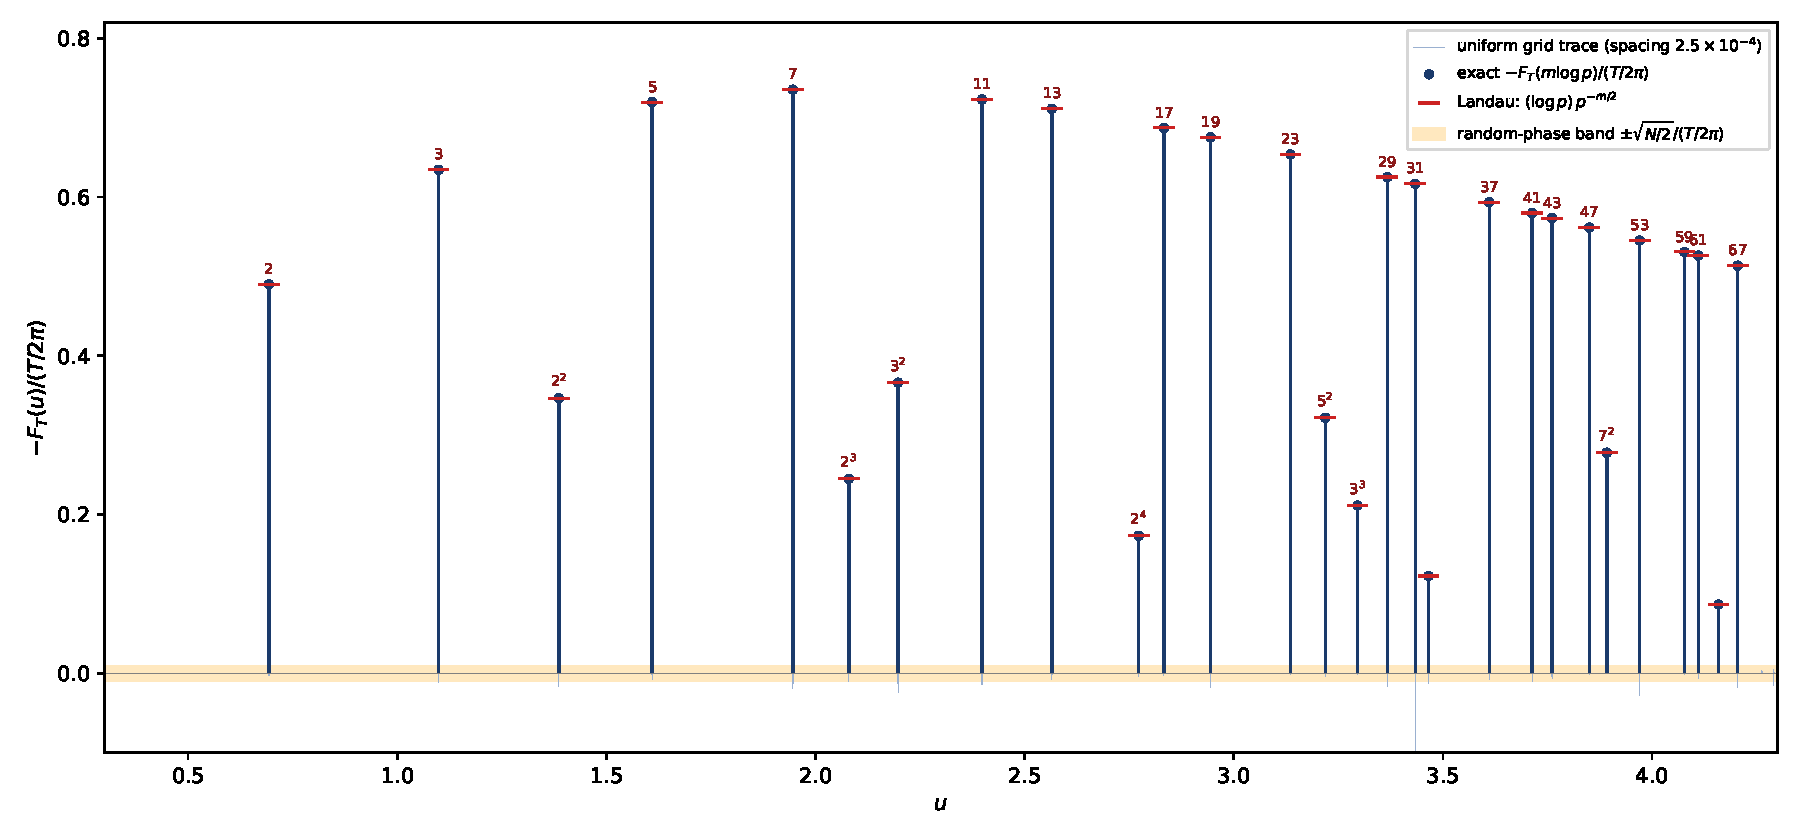
\includegraphics[width=\textwidth]{figures/dyson_diffraction_T400000}
  \caption{Diffraction of the \ladderCount{} certified zeros at $T = \ladderHeight$.
  Stems: exact sums $-F_T(m\log p)/(T/2\pi)$ at the prime-power frequencies
  (labels $p$, $p^m$). Red dashes: the Landau main term $(\log p)\,p^{-m/2}$,
  visually indistinguishable from the stems at every peak. The faint trace is a
  uniform frequency scan, which stays inside the random-phase band (orange)
  away from the prime powers: pure point diffraction. The peaks are
  $\sim T^{-1}$-narrow, so the uniform scan undersamples them; the stems are
  computed exactly at each $m \log p$.}
  \label{fig:diffraction}
\end{figure}

The trust label on this subsection differs from its neighbors, and we state it
plainly: \cref{fig:diffraction} is a \emph{numerical demonstration}, not a
kernel theorem. The summed ordinates are rigorous Arb ball enclosures (width
$\le 3\times10^{-11}$, the same certified-inventory class that gates the band
certificates), but the cosine sum itself is floating-point, and the kernel has
not seen it. What the kernel currently certifies about each zero is its
existence, line position, and a sign-change bracket of width $\sim 0.3$---too
coarse by five orders of magnitude for a certified $233{,}000$-term
trigonometric sum. Closing that gap is mechanical, and staged: a
\emph{refinement pass} bisecting each certified bracket to width $10^{-6}$
(the same IVT machinery, $\sim 21$ extra amortized evaluations per zero); a
\emph{certified cosine} lemma family in Lean (high-order Taylor with explicit
Lagrange remainder, $\pi$-free range reduction by iterated double-angle, plus
the Lipschitz bound $|\cos a - \cos b| \le |a - b|$ to absorb bracket width);
and per-band \emph{partial-sum interval boxes} emitted alongside each band
certificate and tree-folded across bands---the height-chain trick applied to
sums, so the certificate mass stays per-band and parallel. The pilot
instance is \emph{done}: the kernel-verified theorem
\texttt{BraggH100.bragg\_amplitude\_h100} (axioms $\{$\texttt{propext},
\texttt{Classical.choice}, \texttt{Quot.sound}$\}$, no \texttt{sorryAx})
proves that the twenty-nine certified on-line zeros
$x_1 < \cdots < x_{29}$ below height $100$ satisfy
\[
  F_{100}(u^*) \;=\; \sum_{k=1}^{29} \cos(x_k u^*) \;\in\;
  [-7.07809487,\, -7.07805467],
  \qquad u^* = \tfrac{693147}{10^6} \approx \log 2,
\]
an enclosure of width $4\times10^{-5}$ produced by the full pipeline:
Arb-verified sign-change brackets of width $10^{-6}$ per zero, a certified
cosine evaluator that range-reduces \emph{without} $\pi$ (thirty double-angle
steps from Mathlib's order-four bracket---the net error
$\theta^4\cdot\tfrac{5}{96}/2^{2M}$ \emph{decreases} with the reduction depth
$M$, so no high-order Taylor kernel is needed), Lipschitz absorption of the
bracket width, and an interval fold over the twenty-nine terms. The
companion theorem \texttt{bragg\_amplitude\_h100\_complete} closes the
formulation gap: for the \emph{intrinsic} support of zeta's divisor in the
box, given the winding exhaustion data, the diffraction sum over
\emph{every} zero in the box lands in the same interval---the exhaustion
argument forces the support to \emph{equal} the witness set, so the sum is
genuinely over the actual zeros, not an exhibited subset. As the pipeline
scales along the ladder, theorems of the form
$|F_T(m\log p) - A| \le \varepsilon$ constitute, to our knowledge, the
first machine-checked diffraction pattern of the zeta zeros: the finite,
unconditional part of Dyson's picture, with the Guinand--Weil identity of the
previous subsection as the bridge from the certified peaks to the primes.

\subsection{The bridge to Li's coefficients: one weighted engine}

The counting formula and the explicit formula above turn out to be the same
machine read with different test weights, and choosing the weight that Li's
criterion cares about carries the apparatus back to the object this section
opened with. The engine is a single weighted argument principle
(\texttt{analytic\_weighted\_count\_eq\_winding}; CI-axiom-guarded, axioms
$\{$\texttt{propext}, \texttt{Classical.choice}, \texttt{Quot.sound}$\}$): for
analytic $f$ and any holomorphic weight $g$, the weighted boundary winding
equals $2\pi i \sum_{\rho} \operatorname{mult}(\rho)\, g(\rho)$. Weight
$g \equiv 1$ returns the zero-count $N(T)$ of the previous subsections; weight
$g(\rho) = 1 - (1 - 1/\rho)^n$ returns the finite box-sum of Li's summands. The
Riemann--von Mangoldt count and the finite Li-sum are \emph{one functional, two
weights}---not an analogy but the same theorem, instantiated twice.

Two further facts, both kernel-clean, place the coefficients themselves. First,
specializing the finite explicit formula to the Li weight
(\texttt{li\_finite\_explicit\_formula}, derived from
\texttt{rect\_explicit\_formula}) yields the finite, rectangular skeleton of the
Bombieri--Lagarias arithmetic form of Li's coefficients
\cite{bombierilagarias1999}: the weighted zero-sum equals von Mangoldt prime
terms on the right edge plus the boundary integrals, the same diffraction shape
as before but now carrying the Li weight. Second
(\texttt{liCoeff\_isLimit\_partialSums}), the $n$-th coefficient---the Taylor
coefficient of $\xi$ whose nonnegativity is Li's criterion---is the limit of
finite partial sums over finite subsets of the zeros, conditional on two named
analytic inputs (genus-one summability $\sum 1/\lVert\rho\rVert^2$ and the
Hadamard product), left as explicit hypotheses. So $\lambda_n$ is reached as the
exhaustion limit of exactly the finite sums the engine computes. And the two
developments are provably about \emph{one} function: \texttt{xiTele\_eq\_riemannXi}
is a \texttt{ring} identity, so the $\xi$ whose box zero-count the counting
formula computes is the very $\xi$ whose Taylor coefficients characterize RH
(recorded, as a conjunction of the two facts, in
\texttt{rvm\_and\_li\_share\_riemannXi}).

The honesty line is the whole point of stating this, and it is drawn sharply.
These are separate kernel theorems, \emph{deliberately not stitched} into a
claim that the count $N(T)$ determines the coefficients $\lambda_n$. Two
structural seams that once stood between them are now formalized. The
$\xi$-versus-$\zeta$ index mismatch is closed: a finite weighted box-sum over
$\zeta$'s strip zeros is a value-preserving sub-sum of $\xi$'s nontrivial-zero
index (\texttt{zeroFinset\_sum\_via\_nontrivial}, a reindexing). And the
$\xi$-side algebra is complete: the four-way split
$(\log\xi)' = s^{-1} + (s-1)^{-1} + (\log\zeta)' + (\log\Gamma_{\mathbb R})'$
(\texttt{logDeriv\_xiTele\_four\_split}) isolates the Archimedean factor exactly,
reducing it to $\tfrac12\,\psi(s/2)$ with $\psi$ the digamma function.

What remains is then an obstruction we can name precisely---and naming it, we
find it is \emph{route-specific}, not intrinsic. Computed the contour way, the
Bombieri--Lagarias main term $\lambda_n \sim (n/2)\log n$ (the one place the zero
density $dN(T) \sim (1/2\pi)\log(T/2\pi)$ becomes load-bearing) requires the
large-argument asymptotic of the digamma function, $\psi(w) \sim \log w$,
integrated against the concentrating weight $g_n$ and extracted by a saddle-point
argument as the contour grows. That asymptotic is \emph{not in the Mathlib we
build against}: its digamma development carries the special values, the recurrence
$\psi(s{+}1) = \psi(s) + 1/s$, and meromorphy, but nothing at infinity; its
Stirling development has only the discrete factorial form, not the continuous
complex $\log\Gamma$ asymptotic.

But the asymptotic is only forced by the contour. Li's own definition takes the
Taylor route---$\lambda_n$ is a coefficient of $(\log \xi)'$ under the M\"obius
change of variable $z \mapsto 1/(1-z)$, which sends the expansion point $z=0$ to
the \emph{fixed point} $s=1$. Along that route the Archimedean factor is sampled,
with all its derivatives, at $s=1$---never at infinity---so the missing
large-argument asymptotic is simply off the path, replaced by exact local
constants. The base datum is already in the kernel:
$(\log \Gamma_{\mathbb R})'(1) = -(\gamma + \log 4\pi)/2$
(\texttt{logDeriv\_gammaR\_one}, CI-axiom-guarded), from Mathlib's own derivative
of $\Gamma$ at $1$. The route's residual has since been \emph{built}. The polygamma theory Mathlib
lacked is now in the kernel from the ground up: the Gauss--Weierstrass digamma
series (\texttt{digamma\_series}, obtained by log-differentiating the Weierstrass
product $s\,e^{\gamma s}\prod(1+s/n)e^{-s/n} = 1/\Gamma$, with $\gamma$ pinned by
Mathlib's harmonic-minus-log limit), the trigamma value $\psi'(\tfrac12) = \pi^2/2$
(\texttt{deriv\_digamma\_one\_half}, its series summed via Basel), and the higher
$\psi^{(k)}(\tfrac12)$ as exact $\zeta$-value data. A Fa\`a di Bruno expansion of
the composition and a Leibniz rule for iterated derivatives---both filling their
own Mathlib gaps---then assemble the Archimedean coefficient in closed form
(\texttt{taylorCoeff\_Gamma}\(\mathbb{R}\)\texttt{\_leibniz}), and the Li coefficient itself splits, as a
kernel theorem, into its exact parts:
\[
  \lambda_n = \texttt{taylorCoeff}(\mathrm{id})_n
    + \texttt{taylorCoeff}(H)_n
    + \texttt{taylorCoeff}(\Gamma_{\mathbb R})_n
\]
(\texttt{taylorCoeff\_riemannXi\_split}, with $H=(s-1)\zeta$ the analytic
$\zeta$-companion at $s=1$), the last summand being the closed polygamma data. This
is the exact, finite coefficient---built, not asserted.

What that leaves is a single, sharper residual: the \emph{growth} of this
now-explicit sequence, $\lambda_n \sim (n/2)\log n$. That is no longer an absent
complex asymptotic on a growing contour, nor a theory to build---it is one named
asymptotic estimate of a known real sequence of $\zeta$-value constants, and it is
the one place the zero density $dN(T) \sim (1/2\pi)\log(T/2\pi)$ would become
load-bearing. We have the exact coefficient; we do not have---and do not claim---its
asymptotic. As everywhere in this section, \texttt{conjecture1\_proved = False}:
nothing here proves or approaches RH.

For completeness we note one boundary item we deliberately keep out of the
verified list, stated as it is: a Borel--Carath\'eodory theorem is present in the
development but is a \emph{draft}---its constant is not sharp, it is not
axiom-guarded, and it is not yet wired into the region argument, so we do not lean
on it. We flag it rather than let it blur into the verified results above.

\subsection{The reverse program: instruments for Dyson's classification proposal}
\label{sec:mirrormere}

Dyson's proposal runs the diffraction picture backward: classify
one-dimensional quasicrystals, locate the zeta point set in the
classification, and derive zero-localization. The tame one-dimensional case
has recently \emph{closed} in the literature: by the loop
Kurasov--Sarnak $\to$ Olevskii--Ulanovskii $\to$ Alon--Cohen--Vinzant, an
$\mathbb{N}$-valued Fourier quasicrystal is precisely the zero-counting
measure of a Lee--Yang exponential polynomial---and Lee--Yang zeros are real
by construction, so \emph{membership forces reality of support}: exactly the
shape Dyson wanted. The zeta comb, however, sits outside the classified
class, and where it escapes is now a pair of kernel theorems, not folklore: the
prime-log frequency set is dense (hence not Bohr-discrete;
\texttt{primeLogSpectrum\_dense}, unconditional) and the ordinate gaps shrink
below any uniform-discreteness bound (a pigeonhole driver against the
counting formula). On the same footing we have formalized the base of the
classification itself (the Lee--Yang circle bridge and the one-frequency
Kurasov--Sarnak crystalline structure, in Poisson test-function form) and a
first \emph{rigidity theorem in the reverse direction}
(\texttt{twoFreq\_realRooted\_iff}, kernel, both directions): a two-frequency
exponential sum has all zeros on a single horizontal line, and is real-rooted
\emph{iff} its coefficients have equal modulus---reality of support forced by
a dual-side condition, in the smallest honest instance; the
rationally-dependent case reduces, in kernel, to Lee--Yang-on-the-circle.

Two further instruments discipline the search for axioms. A \emph{certified
control zoo}: a rigorous Davenport--Heilbronn driver (ball-arithmetic Hurwitz
evaluation, the mixing constant enclosed from integer surds) yields a
winding-certified zero inventory to height $300$---$204$ on-line, $4$
off-line, correcting two published values along the way (the off-line zero
near $\gamma \approx 166.5$ has $\beta \approx 0.60$, not the tabulated
$0.785$, which our winding count rejects; the tabulated off-line zero near
$\gamma \approx 243.1$ does not exist)---and a mechanized falsification
harness that runs candidate axiom sets against certified data. Its verdict:
the clause that kills DH (which has off-line zeros, so every admissible axiom
set \emph{must} kill it) while zeta's unconditionally-checkable clauses pass
is \emph{weight positivity}---the Euler product---isolated by a
deliberately-dead control variant that DH survives. And a \emph{defect
instrument}: the inertia arithmetic of the finite Weil-form compression
\cite{alpogefurman} (an off-line pair contributes a signature-$(1,1)$ block)
is formalized as a defect dictionary---negative index $\le$ number of
off-line pairs, defect $0$ unconditionally for on-line configurations---and
exercised in a certified perturbation experiment: adjoining one synthetic
off-line pair ($\beta = 3/5$) to the twenty-nine certified zeros below $100$
produces a kernel-observable defect of $-1.00167\times10^{-4}$ against the
honest configuration's $0$. The conservation-of-difficulty map that emerges
is stated plainly in the program documents: positivity, multiplicativity,
density, and the defect arithmetic are unconditional (and now partly
kernel-checked); RH-hardness concentrates in exactly one clause---FQ-grade
temperedness of the dual comb---of which the classification's entrance fee
is the disguise. \emph{None of this proves anything about RH}; it builds the
finite, machine-checked floor---ground truth, falsification instruments, and
the first theorems of the rigidity ladder---on which any serious attempt at
the reverse derivation would have to stand.

\subsection{Reflection, and the return of the classical objects}
\label{sec:reflection}

Every certificate in the ladder of \cref{sec:rh} rests, by design, on one
documented seam: numeric enclosures enter the kernel as \emph{hypotheses},
supplied by ball arithmetic and audited but never re-derived. The
\emph{reflection program} asks whether that seam can be removed---whether the
kernel can \emph{compute} the numerics itself---and this section reports how
far it has gone and what happened along the way. The short answer: the seam
is eliminable in principle and now partially eliminated in fact; and at every
step where the machinery was forced to choose a representation, it chose,
unprompted, a classical object of the subject's history.

The architecture is computational reflection in the standard sense: a
checker \texttt{checkBand : BandData $\to$ Bool} written in the restricted
fragment the kernel evaluates well (integer-mantissa dyadic intervals, list
folds, structural recursion---no rationals, whose GCD normalization defeats
kernel reduction), a soundness theorem proven once, and per-band certificates
of the form \texttt{ok : checkBand d = true := by decide}. The pilot band
landed with an axiom print worth exhibiting: the kernel decision
\texttt{ReflectedBand\_t14.ok} depends on \emph{propext alone}---no choice,
no quotients, no numeric hypotheses---with the classical axioms entering only
downstream, where the soundness bridge converts the decided bit into the
existence of on-line zeros via the intermediate value theorem. The analytic
engine beneath it is a kernel-complete Euler--Maclaurin theory built for the
purpose (and absent from Mathlib): the order-3 identity
\[
  \zeta(s) \;=\; \frac{1}{s-1} + \frac12
  + \int_1^N \widetilde{B}_1(x)\,(-s)x^{-s-1}\,dx
  + \frac{B_2}{2}\,s\,N^{-s-1} + R_3(s,N),
  \qquad 0 < \operatorname{Re} s,\ s \ne 1,
\]
with $R_3$ an explicit saw-kernel integral, culminating in a
\emph{kernel-decided} numeric theorem:
$\lVert \zeta(\tfrac12 + 14i) - \mathrm{emZetaFinite}_3 \rVert \le 10^{-3}$
at $N = 200$ (the proven envelope is $6\times$ smaller). Two smaller
felicities deserve record: the order-3 boundary term vanishes because
$B_3 = 0$---the odd Bernoulli zeros doing concrete labor in a certificate
format---and the large trigonometric arguments the evaluator needs
($\cos(t\log n)$ with $t\log n \approx 74$, a dozen full periods) are reduced
\emph{without any enclosure of $\pi$}: iterated exact halving into the Taylor
domain and doubling back through $\cos 2y = 2\cos^2 y - 1$, the reduction
error \emph{shrinking} geometrically with depth. On these instruments the
first fully unconditional evaluation landed: a no-argument kernel theorem
placing $\operatorname{Re}\, 2^{-(1/2+14i)}$ in an interval of width
$2\times10^{-4}$---to our knowledge the first value of a $\zeta$-series term
on the critical line ever computed, rather than certified, inside a proof
assistant's trusted core. The full $\zeta(\tfrac12+it)$ box is a mechanical
sum of two hundred such terms plus the tail theorem above.

Now the striking part, which we did not design. The remaining factor of
$\Lambda = \Gamma_{\mathbb{R}}\,\zeta$ is the Archimedean one, and the
economical route is not to enclose $\Gamma_{\mathbb{R}}$'s value but to use
the reality of $\Lambda$ on the line: the sign of $\mathrm{gLine}$
decomposes as
$\operatorname{sign}(\cos\varphi\cdot\operatorname{Re}\zeta -
\sin\varphi\cdot\operatorname{Im}\zeta)$ with
$\varphi = \arg\Gamma_{\mathbb{R}}(\tfrac12+it)$, the positive modulus
dropping out. The quantity this leaves behind is precisely the
\emph{Hardy $Z$-function}, and the phase $\varphi$ is precisely the
\emph{Riemann--Siegel theta}: the evaluator, asked only for the cheapest
sound decomposition, reconstructed the instrument of every zero verification
since Hardy, and the reflected campaign converges---from the axioms of type
theory upward---on Turing's own method. The same phenomenon occurred one
level down in the finite models of \cref{sec:mirrormere}: the reality
criterion for a self-inversive exponential sum forces a normalization by a
unimodular \emph{square root} of the functional-equation phase, $u^2 =
\mathrm{phase}$---Hardy's half-phase $e^{i\theta}$, reappearing in a
two-term binomial because the symmetry demands it, not because we put it
there. We take this recurrence seriously as evidence of a correct frame:
when independent mechanized searches for the \emph{cheapest checkable
certificate} keep terminating on the classical objects---$Z$, $\theta$, the
half-phase, the Selberg-class axioms recovered clause-by-clause by
falsification against Davenport--Heilbronn (\cref{sec:mirrormere})---the
suggestion is that those objects are not historical conveniences but
something like the optimal certificates of the theory, rediscoverable by
any sufficiently honest verifier.

One instrument now separates the program from a zero-hypothesis band---a
kernel value for $\theta(t)$ itself. The corpus route (quadrature of the
enclosed $\log\Gamma_{\mathbb{R}}$-derivative) is genuinely blocked: it
requires a digamma series representation and polygamma bounds that exist
nowhere in Mathlib, and we decline to manufacture them mid-campaign. But a
back door stands open, and it is three centuries old: Euler's limit formula
(already formalized in Mathlib as the $\Gamma$-sequence) gives
$\arg\Gamma(z)$ at finite stage $n$ as
$y\log n - \sum_{k\le n} \arctan\!\big(y/(x+k)\big)$---arctangents at
rational arguments, exactly telescoping harmonic sums, and explicit
$O(1/n)$ rates, every ingredient already in the toolkit. That assembly is in
progress as we write. If it closes, the resulting theorem---the existence of
a nontrivial zero of $\zeta$, proven by a term that takes no arguments and
invokes no oracle---would be the natural endpoint of the trust programme
this paper describes: not a verified \emph{account} of a computation, but
the computation itself, carried out where nothing unverified can reach it.
As everywhere: \texttt{conjecture1\_proved = False}; the reflection program
changes what a finite verification \emph{is}, not what it proves.

\subsection{Directions: the uniformization axes}

Every classical route to the Riemann Hypothesis supplies a \emph{uniform
object} together with an equivalence $\mathrm{RH}\Leftrightarrow(\text{the object
holds uniformly})$: positivity of every Keiper--Li coefficient $\lambda_n$
(Li 1997; Bombieri--Lagarias 1999), hyperbolicity of every Jensen polynomial
$J^{d,n}_\gamma$ (P\'olya 1927; Griffin--Ono--Rolen--Zagier 2019), positivity of
the Weil functional on the whole test space (Weil 1952; Bombieri 2000), a
zero-free half-strip reaching $\mathrm{Re}=1/2$, vanishing of the
Nyman--Beurling distance $d_N\to 0$ (Beurling 1955; B\'aez-Duarte 2003), or
self-adjointness of a Hilbert--P\'olya operator. In each case the equivalence
factors as \emph{finite faces plus an infinite quantifier}: a certificate-
compilation engine (untrusted generator, trusted kernel) can discharge the
finite faces---individual rungs, discriminant/Gram/PSD instances, finite-height
identities---but the completion is an infinite conjunction or uniform-in-parameter
statement whose discharge \emph{is} RH. This is the honesty theorem: a complete
uniform certificate exists if and only if RH holds. The six axes are one wall in
six coordinate systems---height-universality, degree-exhaustion, cone-exhaustion,
basis-exhaustion, and spectral-realization---and the confirmed partial results
(Freitas' infinitely-many-negative-$\lambda_n$; GORZ's ineffective threshold
$n_0(d)$ worsening as $d\to\infty$; the $\log T/T$ Weil tail budget; Burnol's
unconditional positive lower bound on $d_N$) show the wall is intrinsic to each
system: changing coordinates changes only what the infinite quantifier ranges
over, never its cardinality. As \emph{program directions}, the highest-value
targets for finite kernel-checked certificate work are the two axes whose rungs
are decidable and shovel-ready: Jensen--P\'olya hyperbolicity (each
$J^{d,n}$ a discriminant/Hermite-PSD certificate, extending the
$d\le 9\times10^{24}$ unconditional range) and finite-window Weil positivity
(reduced by recent work to the PSD-ness of a single explicit Gram matrix,
with a two-sided certification calculus over a certified archimedean-tail
budget). We stress the ceiling explicitly: none of these routes closes RH, each
route's completion is itself the open problem, and $\texttt{conjecture1\_proved}
= \texttt{False}$. The contribution is a verified ladder of finite rungs and the
certification calculus on top of them---never the uniform object, which is RH.

The methodological point for this paper is that the same
untrusted-generator/trusted-kernel discipline that handled a combinatorial
extremal problem also produces honest analytic results---and, just as important,
makes it easy to state exactly how strong they are and are not.

\section{The Telperion system}
\label{sec:system}

Here is the whole idea in one sentence: \emph{you describe a family of concrete
claims, Telperion finds a certificate for each one and writes it out as Lean, and
Mathlib's kernel re-proves every line from scratch.} You never have to trust
Telperion. If it produces a bad certificate, the Lean build fails; it cannot
produce a convincing-but-wrong proof, because the only thing that counts a proof
as finished is the kernel. That inversion---\emph{check the witness, don't trust
the author}---is what lets an untrusted search procedure contribute to a
trustworthy proof.

\subsection{The pipeline}

A Telperion run has four stages.

\begin{description}
  \item[Define.] You write a \emph{family}: a grid of instances sharing a shape,
    each given by its symbols, its parameters, and the inequality (or identity)
    it asserts. This is the only part you author. A family might be ``Bernoulli's
    inequality for $k = 2, \dots, 12$'' or ``this per-cell bound over every
    configuration in a $6 \times 6$ grid.''
  \item[Certify.] Telperion produces an exact witness for each instance---an SOS
    decomposition, a Positivstellensatz multiplier, a rational identity, a
    $p$-adic valuation, whatever the shape calls for. All of this happens in
    \emph{exact} arithmetic (Python's \texttt{Fraction} and \texttt{sympy}); no
    floating point ever touches the certificate path, so ``it certified'' means
    exactly that, not ``it certified up to rounding.''
  \item[Emit.] The certified family is rendered to Lean~4. Each instance becomes
    one theorem with a full proof term, written against a target project you
    describe once (its imports, namespace, and options).
  \item[Freeze.] The emitted file is written with a content hash, and can be
    re-generated and compared byte-for-byte against the committed copy. A drift
    is a hard error---which means the artifact you read is the artifact that was
    checked.
\end{description}

The load-bearing step is the one that isn't ours: after \textbf{emit}, you run
\texttt{lake build}, and \emph{Mathlib's kernel} re-proves everything against a
pinned toolchain (Lean~4 \texttt{v4.32.0} and the matching Mathlib)
\cite{lean4,mathlib}. The generator is untrusted \emph{by design}; the kernel is
the sole trusted component.

\subsection{A worked example, start to finish}

Take Bernoulli's inequality, $(1+x)^k - 1 - kx \ge 0$. As a family it is one
parameter, $k$, over a small grid. Telperion certifies each $k$ by writing the
left-hand side as a manifestly nonnegative combination, emits a Lean theorem per
$k$, and---once you run \texttt{lake build}---the kernel checks each proof term.
The entire example is a single self-contained script,
\texttt{examples/bernoulli/generate.py}; running it writes
\texttt{lean/BernoulliSolution.lean}, and \texttt{lake build} in that directory
is the proof. You are welcome to read the emitted Lean, but you do not have to:
edit any constant in it and the kernel rejects the file. That is the guarantee in
miniature.

\subsection{What it can prove}

Telperion is not tied to one kind of certificate. It carries roughly eighty
emitters---one per certificate \emph{shape}---spanning a broad slice of concrete
mathematics. \Cref{tab:shapes} groups a representative sample; the point is not
the exact count but the range: the same untrusted-generator/trusted-kernel
discipline covers textbook inequalities, semialgebraic positivity, integer
rounding, and combinatorial and analytic certificates alike.

\begin{table}[t]
  \centering
  \begin{tabular}{@{}ll@{}}
    \toprule
    Family & Representative shapes \\
    \midrule
    General / textbook & rational-function inequalities, exact identities,
      P\'olya positivity \\
    Semialgebraic positivity & SOS (with Artin denominators), Handelman, Putinar,
      Nullstellensatz \cite{positivstellensatz,lasserre_sos} \\
    Discrete / arithmetic & Chv\'atal--Gomory integer rounding, $p$-adic
      valuations, finite case analysis \\
    Analytic & zero-free-region atoms, half-plane/disk bounds, transcendental
      enclosures \\
    Combinatorial (this campaign) & tight-cap enclosure, cavity/recursion
      closure, curvature-boundary extrema \\
    \bottomrule
  \end{tabular}
  \caption{A representative sample of Telperion's certificate shapes. For the
    positivity shapes, an automatic search (a P\'olya engine, plus optional SDP
    finders) will often construct the certificate for you.}
  \label{tab:shapes}
\end{table}

\subsection{Reproducibility}

Because the generator is untrusted, reproducibility has teeth. Every emitted file
regenerates byte-for-byte (\texttt{generate.py -{}-check} is the drift gate), and
continuous integration compiles the emitted Lean against the pinned Mathlib on
every change. A reviewer does not have to take our word for any of it: the recipe
to regenerate a certificate and re-run the kernel check is a handful of commands,
given in the reproducibility appendix, and the CI status badges are standing
evidence that the checks are green.

\subsection{The vacuity gap and self-verification}
\label{sec:vacuity}

The kernel is a strong guarantee, but it is important to be precise about what it
guarantees. The kernel certifies that a proof term proves \emph{its stated
theorem}. It does not certify that the stated theorem is the one you meant, nor
that the theorem says anything at all. A theorem can be true and yet
\emph{vacuous}---$X = X$ proves nothing, and a more subtle relative can hide the
same emptiness behind real-looking algebra. The kernel will happily accept it.
This is the one gap Telperion is built around, and we would rather name it
loudly than paper over it.

\subsection{Making emitters declare themselves}

Every emitter must declare a \emph{sensitivity stance}, and a test refuses to let
one ship without it:

\begin{itemize}
  \item \textbf{Certificate-sensitive.} The emitted theorem carries a corruptible
    witness---a specific numeric or algebraic identity that is doing the work. For
    these, a wrong witness must break the proof. We check exactly that with a
    \emph{negative control}: forge the witness and confirm the kernel
    \emph{rejects} the forgery. If corrupting the certificate still compiles, the
    certificate was not load-bearing, and the emitter is refused.
  \item \textbf{Structurally non-vacuous.} The theorem is a positivity,
    decidability, finite-cover, or hypothesis-gated statement with no separable
    corruptible witness. Here a structural non-vacuity check---run at emit time,
    refusing reflexive and trivial statements---is the right guard, and the
    contributor writes one line saying why.
\end{itemize}

The distinction is not bureaucracy; it is the difference between ``the kernel
accepted a proof'' and ``the kernel accepted a proof that could have failed.''
Only the second is evidence.

\subsection{A second, independent kernel}

For an even stronger check, Telperion integrates an independent judge: the
Comparator \cite{comparator}, drawn from OpenAI's ten-proofs project
\cite{tenproofs}, together with \texttt{nanoda}, a from-scratch reimplementation
of the Lean type checker in Rust \cite{nanoda}. The Comparator confirms that an
emitted proof proves \emph{exactly} the challenge statement using only a
whitelisted set of axioms. Two independently written checkers agreeing is a
meaningfully higher bar than one.

\subsection{The gap, encountered in the wild}

This is not a hypothetical hazard for us; it visited this very campaign. Midway
through the counting-formula program (\cref{sec:rh}), a planning claim---``this
entire function carries the nontrivial zeros''---was simply false, while every
kernel theorem built around it remained true: the reflection identities were
correct statements about the wrong object. The kernel could not have caught it,
because the false claim lived in docstrings and plans, not in any theorem. It
was caught one step later by checking the premise against Mathlib's own
defining identity, the detour was relabeled rather than hidden, and the durable
fix is the one this section recommends in general: the successor object's zero
set was not asserted but \emph{proved}, as an iff, in the axiom guard. The
kernel guards statements; the discipline must guard what the statements are
about.

\subsection{The gap, encountered a second time---and caught by the machinery}

A harder instance arrived during the Turing-ladder campaign (\cref{sec:rh}),
and this time the discipline of this section, not luck, caught it. The original
winding-route band certificates carried an edge-hypothesis bundle of the shape
``for every decomposition of the boundary data satisfying $P$, the interior
zeros are confined''---universally quantified over a decomposition that the
intended Arb data was supposed to instantiate. Auditing the shape before
scaling the campaign, we asked the sensitivity question this section mandates:
\emph{what else satisfies the premise?} The answer was: junk. A decomposition
padding the zero multiset with a phantom point of multiplicity zero, or
absorbing an off-ball point into the error term, satisfies $P$ while violating
the confinement clause---so the bundled hypothesis was false for every band,
the per-band theorems true but \emph{vacuous} as certificates, and the
milestone claims built on them empty. The kernel had accepted every one of
them, because every one of them was true. Three consequences followed, each the
recommendation of this section made concrete. First, the affected milestone
claims were \emph{suspended publicly}, in the pull request and the campaign
document, the day the vacuity was found. Second, the replacement certificate
shape was made \emph{canonical and audited}: every re-based band instantiates
one fixed Prop (\texttt{TuringBand.BandStatement}) whose shape is pinned by
hand-audited kernel code, so an emitter can vary only parameters that are
numerically cross-checked, and a kernel statement-match gate plus
forge-the-witness negative controls run over every band in continuous
verification. Third, the entire ladder---every zero of every prior
milestone---was re-verified on the new shape before any claim was reinstated;
the re-based census agrees with the rigorous count $N(T)$ exactly at every
thousand-block. The episode cost one day. Scaling a quarter-million-zero
verification on a vacuous certificate shape would have cost the paper.

\subsection{The floor we cannot get under}

Honesty requires stating the limit, too. No amount of machinery decides whether a
\emph{formal} statement faithfully captures the \emph{informal} claim a human had
in mind; that correspondence lives outside any formal system, and by the usual
self-reference obstructions (L\"ob, G\"odel) it cannot be internalized. So the
irreducible trusted component is not Telperion and not even the kernel---it is the
human reading of the theorem statements. Everything in this section shrinks the
untrusted surface down to that floor; nothing can remove the floor itself. We
take that as a reason to keep the statements short, legible, and few, not as a
reason to pretend the floor is not there.

\section{Evaluation and limitations}
\label{sec:evaluation}

We would rather this section be read as a list of caveats than as a victory lap,
because that is the honest shape of the work.

\paragraph{Novelty is claimed conservatively.} Where we say a result may be the
first of its kind---the machine-checked Hadamard-free zero-free regions, the
symbolic-in-$n$ proof-complexity lower bound---we mean it as a careful,
literature-searched belief, not a settled priority claim. The repository's
publication ledger states novelty provisionally and un-lit-checked by design, and
we carry that same conservatism here. The contributions we are confident about are
the \emph{system} and the \emph{formalizations}; the underlying mathematics in the
case studies is, in each case, attributed to its originators.

\paragraph{What the tool does not do.} Telperion does not choose your problem or
your family; it certifies instances of a shape you supply. It does not search for
the right theorem to prove, and it offers no guarantee that a certificate exists
for a claim that is true---only that if it emits one, the kernel will confirm it.
And, as \cref{sec:vacuity} argues, it cannot close the gap between a formal
statement and the informal claim a human intended; that reading is the irreducible
trusted floor.

\paragraph{What would falsify our claims.} The claims in this paper are
deliberately falsifiable. Every ``verified'' assertion names a Lean theorem
checked against pinned Mathlib with a clean axiom set; a reader who rebuilds the
project and finds a \texttt{sorryAx}, an added axiom, or a statement that does not
say what we claim it says has refuted the corresponding claim. The reproducibility
appendix gives the commands. We regard that exposure as the point, not a risk.

\section{Related work}
\label{sec:related}

Telperion stands on Lean~4 and its mathematical library, Mathlib
\cite{lean4,mathlib}: the emitted proofs are Lean, and the kernel that checks them
is Lean's. The idea of producing a checkable certificate rather than trusting a
procedure is the reflection/certificate tradition in proof assistants, and in the
positivity setting specifically it goes back to Positivstellensatz and
sum-of-squares certification \cite{positivstellensatz,lasserre_sos}, which several
of Telperion's shapes emit.

Two recent efforts from Axiom Math are close in spirit, and we want to keep them
distinct because they are distinct projects. \emph{AXLE} \cite{axle} is a cloud
Lean-verification utility; we drew engineering patterns (verification, gap-filling,
repair, negative controls) from it, but no code. \emph{AxiomMath/ZetaZeros}
is a Lean formalization of a pair-correlation zero-simplicity result of Lamzouri
\cite{axiommath_zetazeros}; two of Telperion's emitters port a \emph{proof idea}
from that formalization---a Montgomery--Taylor extremum-at-the-boundary move and a
transcendental enclosure atom---independently re-implemented in our idiom. Conflating the
verification utility with the formalization would misattribute both; the
repository's \texttt{NOTICE} file records the split in full.

The framing of this paper stands on a classical lineage we want to cite
plainly. The explicit formula connecting zeros to primes descends from
Riemann's memoir through Guinand \cite{guinand1948} and Weil \cite{weil1952};
the quasicrystal reading of that identity---the zeros as a one-dimensional
point set with pure-point diffraction on the prime powers, and the suggestion
that classifying such sets is a road toward RH---is Dyson's \cite{dyson2009}.
Our contribution to that lineage is deliberately modest and precisely scoped:
the \emph{finite-height} form of the identity, and the supporting localization
and region results, as kernel-checked certificates. The classical analytic work
of estimating boundary terms and passing to limits is not re-done here, and the
classification program itself we leave exactly where Dyson left it.

For independent checking, we use the Comparator \cite{comparator} from OpenAI's
ten-proofs project \cite{tenproofs}, together with \texttt{nanoda} \cite{nanoda},
a from-scratch Lean type checker in Rust; agreement between independently written
checkers is the basis of our strongest confidence claim. In the results and excursion sections, the
mathematics is due to others and cited there: Brualdi and Goldwasser for the tree
problem \cite{brualdi1984}; de la Vallée-Poussin for the classical zero-free region
\cite{dlvp1896}; Grigoriev and Laurent, with the symmetric-SOS technique of
Kurpisz, Lepp\"anen and Mastrolilli, for the proof-complexity lower bound
\cite{grigoriev2001,klm2016}.

\section{Conclusion}
\label{sec:conclusion}

Dyson's quasicrystal picture asks us to see the zeros of the zeta function as a
diffraction pattern---an aperiodic point set whose spectrum is the primes. This
paper's contribution to that picture is the part a kernel can hold today, and
it has a shape worth stating plainly: first where the zeros \emph{cannot} be
(zero-free regions, up to an effective de la Vallée-Poussin constant), then
where they \emph{are} (all $649$ of them to height $1000$, exactly on the
line), and finally what they \emph{mean} (the finite-height explicit formula,
under which the zeros diffract off the primes). Exclusion and identity---the
two halves of understanding a point set---now live in the same kernel, under
the same three axioms, with the same honest flag flying over both:
\texttt{conjecture1\_proved = False}, until the mathematics itself says
otherwise.

The instrument matters as much as the results, because it is why the results
can be believed at this scale. Telperion is a small idea taken seriously: if a
generator hands you a certificate instead of an argument, you can accept its
work without trusting it, because a trusted kernel re-checks the certificate
from scratch. Built into a tool---with a self-verification layer for the one
thing a kernel cannot see, and an explicit account of the one thing no
machinery can settle---that idea scales to hundreds of kernel-checked theorems,
and it carries across subjects: the same discipline that assembled the
diffraction identity also machine-checked the analytic core of a 42-year-old
extremal tree conjecture (still open, with the missing bridge named) and a
symbolic-in-$n$ lower bound in proof complexity (where the mathematics is
someone else's).

The road ahead is marked rather than promised: estimating the explicit
formula's boundary terms and sending the box to its limits; extending the
Turing verification beyond height $1000$, which the band-tiled architecture
makes a driver exercise rather than a proof; and letting the finite identity
meet concrete test functions and real prime data. In each case the interesting
content and the honest boundary will be stated in the same breath---which is
exactly what a certificate engine, whose value is that you need not trust it,
ought to make easy. The open fronts stay open; we would rather leave them
clearly marked than quietly filled.

\section*{Epilogue: the windowpane}

There is a popular image of the Riemann Hypothesis, fixed on film: John Nash,
alone in a Princeton library, writing on a windowpane---one mind against the
problem, the mathematics as marks on glass, sustained by nothing but conviction.
The real history is harsher than the image. Nash did go after the Riemann
Hypothesis, in the late 1950s, and his 1959 lecture on it at Columbia is
remembered as the moment his audience understood that something had gone
wrong \cite{nasar1998}. He is not the only brilliant mind that problem has
asked too much of. There is a long, quiet ledger of people who stared into the
critical strip alone, holding an entire argument in one head, with nothing
outside themselves to say which steps were real.

The method of this paper is, in one sense, an answer to that image. Nash wrote
\emph{on} the glass; here the glass \emph{is} the mathematics. Each pane is a
band certificate whose winding count was computed twice and checked by a
kernel; the leading between panes is a contour the kernel re-proved from
scratch; and the light through the window---the primes---needs no certificate
at all, because on $\operatorname{Re} s > 1$ the Euler product makes
non-vanishing a theorem. It is a Princeton window in more ways than one: it was
in the Institute's tea room that Montgomery showed Dyson the pair correlation
of the zeros and Dyson recognized the random-matrix kernel at sight
\cite{montgomery1973}, and it is Dyson's later quasicrystal reading of the
zeros \cite{dyson2009} that gives this paper its title and the window its
geometry.

The quiet property of the certificate method---quieter than any theorem in
this paper, and perhaps worth more---is that \emph{conviction is not
load-bearing}. A wrong step here is a compile error, never a false belief
carried forward; a hard night degrades throughput, never truth; and the flag
\texttt{conjecture1\_proved = False} is not a disclaimer bolted on at the end
but the design principle the whole instrument is built around. No one working
this way has to hold the entire argument alone, and no one has to break
against the problem to work on it. The conjecture stands, as it stood for
Nash. What has changed is not the summit but the manner of the climb:
witnessed, checked, and shared. The window holds whether or not the mason is
at his best---and that, in the end, is what the leading is for.

A word, finally, about who the masons were, because this paper was produced
by a human--machine collaboration of a kind the community is right to
scrutinize. There is a legitimate fear abroad: that machine-generated
mathematics will bury insight under correctness---results true in the
kernel's eyes and opaque in everyone else's, the discovery of new concepts
choked off in obscurity of code. We lived inside that question for the whole
of this work, and the evidence we can offer cuts the other way, on three
counts. First, the fear has a technical name---the vacuity problem, a true
theorem that does no work---and it is answerable by engineering: every
discipline in \cref{sec:vacuity} (statement gates, forged-witness controls,
sensitivity declarations) exists precisely so that machine speed can never
outrun human meaning. Second, and to us most striking: at every point where
the machinery was free to choose any representation that would check, it
converged, unprompted, on the classical inheritance---Hardy's $Z$, the
Riemann--Siegel phase, the half-phase normalization, the Selberg axioms
recovered clause by clause by falsification (\cref{sec:reflection}). The
concepts were not paved over; they were \emph{rediscovered from below},
which suggests they were never fragile ornaments of human culture but
attractors in the space of honest certificates---findable by any verifier
sufficiently constrained to tell the truth. Third, the division of labor was
real and neither party's contribution was dispensable: the questions that
redirected the program at its hinges---what does the symmetry say; where is
the torus; does this not beg recurrence---were human questions, and the
bridges crossed in answer, at a complexity no unaided human could compute
and an honesty no unaided intuition could enforce, were built jointly and
checked by a third party neither collaborator can charm. Human meaning,
machine reach, kernel truth: the triangle held for every theorem in this
paper. We offer it not as a threat to the working mathematician but as what
it felt like from inside---a wider window, more leading, more light.


\appendix
\section{Reproducibility}
\label{sec:reproducibility}

Every ``verified'' claim in this paper can be re-checked from a clean machine. The
recipe below regenerates a certificate and re-runs the Lean kernel on it; the same
pattern applies to every example in the repository.

\paragraph{Generate (Python only).}
\begin{verbatim}
  pip install -e telperion
  cd telperion
  python examples/bernoulli/generate.py         # writes lean/BernoulliSolution.lean
  python examples/bernoulli/generate.py --check  # confirms byte-stable regeneration
\end{verbatim}

\paragraph{Verify (the Lean kernel).} This is the step that makes it a proof. It
needs the pinned toolchain (Lean~4 \texttt{v4.32.0}, installed automatically by
\texttt{elan}) and a prebuilt Mathlib cache---not a from-source Mathlib build:
\begin{verbatim}
  cd telperion/examples/bernoulli/lean
  lake exe cache get    # prebuilt Mathlib oleans (minutes, not hours)
  lake build            # the kernel re-checks every emitted theorem
\end{verbatim}
A clean exit means the kernel accepted every proof term. Edit any constant in the
emitted \texttt{.lean} and \texttt{lake build} rejects it---the guarantee in
miniature.

\paragraph{Standing evidence.} Continuous integration runs exactly these checks on
every change: it compiles the emitted Lean against pinned Mathlib and, for the
axiom-guarded results, runs \texttt{\#print axioms} and fails on any
\texttt{sorryAx} or added axiom. The status badges on the repository are the
at-a-glance record that the kernel checks are green. Full setup instructions,
including the case-study libraries, are in the repository's Telperion
getting-started guide.

\section{The Telperion compendium: emitter catalog and subsystems}
\label{sec:compendium}

This appendix is a \emph{dated snapshot}---2026-09-09, at 126 emitter
modules---of a catalog that grows by design; the authoritative, current
registry is the repository itself (every emitter must register a sensitivity
stance, \cref{sec:vacuity}, and a test refuses shipment without one, so the
in-repo list is complete by construction). Several modules house small families
of related kinds; the campaign-specific drivers of \cref{sec:rh} (box,
empty-band, on-line sweep) emit through the shapes below. Descriptions are
condensed from each emitter's own docstring.

\subsection{Emitter catalog}

\begin{longtable}{@{}p{0.34\textwidth}p{0.60\textwidth}@{}}
\toprule
\textbf{Kind} & \textbf{What it certifies} \\
\midrule
\endhead
\bottomrule
\endfoot
\multicolumn{2}{@{}l}{\emph{Algebraic and textbook inequalities}} \\
\texttt{identity} & exact identities / equalities (the equality half of a campaign) \\
\texttt{rational\_identity} & rational-function identities over $\mathbb{Q}$ on a ray \\
\texttt{consequence} & equations following from polynomial hypotheses \\
\texttt{tangent} & tangent-line trick for symmetric-sum inequalities \\
\texttt{cauchy\_schwarz} & Cauchy--Schwarz / QM--AM via pairwise-difference SOS \\
\texttt{bernstein} & Bernstein-basis positivity on a closed interval \\
\texttt{sturm\_positive} & strict interval positivity via Sturm chains \\
\texttt{logconcave} & log-concave single-point reductions \\
\texttt{turan\_box} & Tur\'an-style log-concavity $a_1^2 \ge a_0 a_2$ over a box \\
\texttt{unimodal} & integer maxima of unimodal sequences \\
\texttt{telescope} & telescoping-potential induction steps \\
\texttt{fwd\_telescope} & forward-difference telescoping (the W2 prover) \\
\texttt{second\_order} & closed forms for three-term linear recurrences \\
\texttt{ratio\_telescope} & multiplicative telescoping of per-step ratio bounds \\
\texttt{monomial\_ladder} & one smallness budget absorbing a monomial ladder \\
\texttt{rpow\_budget} & $k$-power product collapse with exponent-level budgets \\
\texttt{two\_row\_solve} & solution-entry bounds for $2\times2$ scalar systems \\
\texttt{separable\_convex} & extrema of separable convex sums \\
\texttt{concave\_stationary\_max} & stationary points of strictly concave objectives as maxima \\
\texttt{scale\_invariance} & homogeneity / objective-degeneracy certificates \\
\texttt{monotone\_tail} & monotone-ratio family tails ($b(s) \le B$ for $s \ge s_0$) \\
\texttt{wz} & WZ / Zeilberger creative-telescoping certificates \\
\texttt{logconvex\_interp} & zero-tolerant log-convexity endpoint interpolation \\
\texttt{multilinear\_perturbation} & Leibniz telescoping $|\prod F - \prod G| \le C\eta$ with exact envelope \\
\texttt{poly\_geom\_closure} & uniform $\sum p(n) r^n \le B$ via synthesized remainder invariants \\
\texttt{gevrey\_majorant} & Gevrey-2 factorial-majorant calculus \\
\texttt{coefficient\_mass} & $\ell^1$-coefficient sup-envelope evaluation \\
\texttt{affine\_ledger} & multi-parameter affine gain/increment ledgers over a box \\
\texttt{finite\_prefix\_absorption} & eventually-bounded $\Rightarrow$ globally-bounded absorption \\
\texttt{continuous\_barrier} & open--closed continuity bootstrap barriers \\
\addlinespace
\multicolumn{2}{@{}l}{\emph{Semialgebraic positivity}} \\
\texttt{rational\_sos} & SOS with Artin/Reznick denominators \\
\texttt{sos\_sdp} & first-class SOS via SDP, exact-rationalized \\
\texttt{putinar} & constrained positivity (Putinar Positivstellensatz) \\
\texttt{handelman} & positivity on polytopes (Handelman) \\
\texttt{cone} & Farkas / nonnegative-combination certificates \\
\texttt{nonneg\_orthant} & positivity on the nonnegative orthant \\
\texttt{domain\_to\_orthant} & constrained domains via affine maps to the orthant \\
\texttt{polya\_zeros} & homogeneous P\'olya certificates tolerating boundary zeros \\
\texttt{lattice\_box} & $d$-dimensional integer Positivstellensatz \\
\texttt{psd\_form} & deterministic PSD certificates for quadratic forms \\
\texttt{spectral\_factorization} & Fej\'er--Riesz: nonnegative trig polynomial $\to$ exact SOS \\
\texttt{bilinear\_corner} & worst-corner positivity of bilinear boxes \\
\texttt{polytope\_max} & multi-affine corner maxima in general dimension \\
\texttt{box\_robust} & $\forall$-box separable-quadratic nonnegativity \\
\texttt{finite\_argmax} & a designated winner strictly beats a finite list \\
\texttt{nullstellensatz} & ideal membership: a polynomial vanishes on a variety \\
\texttt{real\_nullstellensatz} & vanishing on the real variety \\
\texttt{infeasible} & Nullstellensatz refutations of polynomial systems \\
\texttt{sos\_refutation} & SOS-Positivstellensatz refutations of semialgebraic systems \\
\addlinespace
\multicolumn{2}{@{}l}{\emph{Discrete and arithmetic}} \\
\texttt{cg\_round} & Chv\'atal--Gomory integer rounding (VIPR-style) \\
\texttt{valuation} & $p$-adic valuation certificates \\
\texttt{finite\_decide} & guarded $\forall$-facts over explicit tables by \texttt{decide} \\
\texttt{integrality\_gate} & finite exceptional tables plus uniform $p$-adic gates \\
\texttt{primality} & Pratt/Lucas primality certificates \\
\texttt{admissible\_tuple} & prime-gaps admissible tuples, decide-checked \\
\texttt{quadratic\_irrational} & $\mathbb{Z}[\sqrt d]$ conjugate-norm separation \\
\texttt{sqrt\_root\_elimination} & symbolic radical elimination \\
\addlinespace
\multicolumn{2}{@{}l}{\emph{Complex analysis: bounds, regions, enclosures}} \\
\texttt{bracket} & rational enclosures of transcendental constants \\
\texttt{transcendental\_enclosure} & rational lower/upper bounds for transcendental values \\
\texttt{algebraic\_bracket} & two-sided enclosures of square roots \\
\texttt{zero\_free\_cosine} & nonnegative-cosine-polynomial zero-free regions \\
\texttt{mt\_cosine} & optimal Mossinghoff--Trudgian cosine polynomials \\
\texttt{lfunction\_product} & the $3$-$4$-$1$ product lower bound \\
\texttt{zero\_free\_region} & zero-free-region assembly \\
\texttt{logderiv\_region} & de la Vall\'ee-Poussin log-derivative region cores \\
\texttt{dirichlet\_repr} & Euler--Maclaurin / Abel-summation representations \\
\texttt{sphere\_bound} & strip growth bounds made uniform on spheres \\
\texttt{halfplane\_disk} & half-plane to disk positivity (M\"obius--Schwarz) \\
\texttt{bc\_deriv\_re} & Borel--Carath\'eodory + Cauchy derivative bounds \\
\texttt{bc\_split} & log-derivative split-plus-entire-bound combines \\
\texttt{borel\_caratheodory} & the Borel--Carath\'eodory bound (upstream packaging) \\
\texttt{cauchy\_deriv} & Cauchy derivative estimates on disks \\
\texttt{max\_modulus} & maximum-modulus propagation to disks \\
\texttt{entire\_part\_bound} & entire-part log-derivative oscillation bounds \\
\texttt{log\_product\_bound} & zero-factor magnitude bounds (two-scale) \\
\texttt{two\_scale\_separation} & inner-disk / outer-sphere separation \\
\texttt{far\_pole\_sum} & rational sums with poles outside the disk \\
\texttt{herglotz\_lower} & Herglotz lower bounds (keep the equal-height zero) \\
\texttt{endpoint\_geom\_cap} & entire-part geometric factors capped at endpoints \\
\texttt{log\_combination} & $F^*$-folding log combinations \\
\texttt{log\_eps\_optimize} & cutoff-parameter optimization for log-eps witnesses \\
\texttt{curvature\_boundary} & sign-definite $f''$ forces extrema to the boundary \\
\texttt{dominated\_integrability} & integrability by rpow domination \\
\texttt{parametric\_holomorphy} & analyticity of parametric tail integrals \\
\texttt{preconnected\_cover} & preconnectedness by convex covers \\
\addlinespace
\multicolumn{2}{@{}l}{\emph{Argument principle and zero localization}} \\
\texttt{winding\_count} & numeric winding cores with kernel emission \\
\texttt{xi\_line\_zeros} & on-line zero counts via sign changes and the IVT \\
\texttt{box\_localization} & the RH-in-a-box counting capstone \\
\texttt{rect\_argument\_principle} & Cauchy vanishing on box boundaries \\
\texttt{rect\_winding} & the winding-nonzero primitive, from scratch \\
\texttt{argument\_principle} & the winding/residue bridge on circles \\
\texttt{full\_argument\_principle} & residue sums plus analytic vanishing in one theorem \\
\texttt{annulus\_count} & zero counts in shells (two-circle difference) \\
\texttt{box\_residue\_sum} & box residue sums conditional on winding \\
\texttt{order\_residue} & order as the residue of the log-derivative \\
\texttt{order\_balance} & integer order boundary contradictions \\
\texttt{jensen\_zero\_count} & Jensen-style zero-count bounds in disks \\
\texttt{slit\_loop\_winding\_zero} & the homotopy-free heart of Rouch\'e \\
\texttt{reexport} & upstream Lean theorems wrapped as named, guarded lemmas \\
\addlinespace
\multicolumn{2}{@{}l}{\emph{RH criterion prefixes}} \\
\texttt{hyperbolicity} & real-rootedness of quadratics over boxes \\
\texttt{jensen\_polynomial\_hyperbolicity} & degree-2 Jensen polynomial hyperbolicity, compile-gated \\
\texttt{interlacing} & Newton log-concavity / real-rootedness \\
\texttt{li\_positivity} & finite rungs of Li's criterion onto the formalized iff \\
\texttt{lee\_yang\_stable\_pair} & Schur stability; zeros-on-a-line by construction \\
\addlinespace
\multicolumn{2}{@{}l}{\emph{Brualdi--Goldwasser campaign}} \\
\texttt{affine\_param\_endpoint} & price-interval collapse to two endpoints \\
\texttt{cavity\_exchange} & Kelmans de-branch monotonicity corner reductions \\
\texttt{recursion\_closure} & per-hub node-decouple recursion closures \\
\texttt{per\_size\_dominance\_sweep} & finite per-$n$ configuration sweeps \\
\texttt{tight\_cap\_enclosure} & fixed-config $g$-step closure faces \\
\texttt{achievability} & achievability-corrected relaxations \\
\texttt{reparam\_adapter} & reparameterization and case-dispatch adapters \\
\texttt{domination\_ratio} & template-dominates-competitor ratio certificates \\
\addlinespace
\multicolumn{2}{@{}l}{\emph{Proof complexity}} \\
\texttt{pe\_duality} & pseudo-expectation / SOS-duality: no degree-$d$ refutation exists \\
\texttt{xor3\_moment} & 3-XOR moment-matrix PSD via block-rank-one SOS \\
\texttt{symmetric\_quad} & symbolic-in-$n$ completing-the-square PSD \\
\texttt{symmetric\_quad\_d2} & the degree-2 symbolic-in-$n$ three-piece variant \\
\texttt{twopoint\_moment} & two-point discrete-measure moment feasibility witnesses \\
\addlinespace
\multicolumn{2}{@{}l}{\emph{Mined from external formalizations (attributed in NOTICE)}} \\
\texttt{two\_moment\_count} & Hermitian moment/inertia count certificates (zeta-23-lean) \\
\texttt{rayleigh\_gram} & generalized-eigenvalue Gram shadows (Axiom bgp212) \\
\texttt{polytope\_moment} & exact-rational simplex moments (Axiom bgp212) \\
\texttt{spacing\_tail\_bound} & concrete spacing-tail instances (zeta-23-lean) \\
\texttt{autocorr\_support} & support-geometry autocorrelation facts (zeta-23-lean) \\
\texttt{enclosure\_interval\_fold} & interval-fold enclosures (zeta-23-lean) \\
\texttt{reflection\_halving} & finite reflection halvings (zeta-23-lean) \\
\addlinespace
\end{longtable}

\subsection{Subsystems (the skills behind the catalog)}

\paragraph{Pipeline core.} Certification in exact arithmetic
(\texttt{certify}), Lean emission against a described target project
(\texttt{emit}), byte-stable freezing with drift detection, statement-match
checking, and provenance headers on every generated file.

\paragraph{Self-verification.} The per-emitter sensitivity registry with
forge-the-witness negative controls (\cref{sec:vacuity}); the independent
Comparator + \texttt{nanoda} second-kernel check; coverage and circularity
audits; a self-hosting layer that applies the discipline to Telperion's own
metatheory.

\paragraph{Certificate search.} A P\'olya engine and optional SDP finders
(exact-rationalized), SONC/AM-GM backends, repair and relaxation passes that
strengthen a failing certificate rather than silently weakening the claim.

\paragraph{Numeric drivers.} Outward-rounded interval arithmetic (Arb) behind
every numeric hypothesis: the box-localization driver (winding counts, edge
non-vanishing, on-line sweeps), the winding-$0$ empty-band driver, and
enclosure generators---all emitting their inputs as \emph{explicit, documented
Lean hypotheses}, never silent constants.

\paragraph{Mining and monitoring.} Certificate-shape mining over external
formalizations (the zeta-23-lean, Navier--Stokes/Euler, and Axiom-bgp212
passes; attributions in \texttt{NOTICE}); a Palomar-registry poller and
arXiv/GitHub/Zulip source monitors that surface new formalizations as emitter
candidates.

\paragraph{Interfaces.} A CLI, an MCP server, and an editor plugin expose the
same pipeline; continuous integration compiles every emitted artifact against
pinned Mathlib and runs the axiom guards on every change.

\bibliographystyle{plain}
\bibliography{references}

\end{document}
